\label{sec:LHC}
The LHC~\cite{LHC}, located at CERN near Geneva, is capable of colliding protons and lead ions at higher energies than any of its predecessors. The instantaneous luminosity delivered to the experiments exceeds that of any previous machine at the energy frontier. It was constructed in the tunnel formerly inhabited by the LEP electron-positron collider in about $\unit{100}{\meter}$ depths below the surface with a circumference of $\unit{27}{\kilo\meter}$. The design goal was to achieve proton collisions at a centre-of-mass energy of $\sqrt{s} = \unit{14}{\tera\electronvolt}$ with instantaneous luminosities of $\unit{10^{34}}{\reciprocal\second\meter\rpsquared}$. 

The LHC consists of eight arcs, as shown in Figure~\ref{fig:LHC}, where superconducting dipole magnets provide a magnetic field of up to $\unit{8.3}{\tesla}$ to bend the charged particles along the curvature of the tunnel, while quadrupole and other specialised magnets are used to focus the beams. In straight segments between these arcs, LHC infrastructure and the experiments are located. The infrastructure components include the cooling facilities necessary to reach a temperature of $\unit{1.9}{\kelvin}$ around the ring, the superconducting cavities in which the protons are accelerated by standing electromagnetic waves, collimators for beam cleaning, and the beam dump, where the beams are ejected from the LHC at the end of fills. In the other four straight segments the beams are brought into collisions, which are studied by the four large experiments at the LHC. Of these, CMS~\cite{CMS} and ATLAS (A large LHC apperatus)~\cite{ATLAS} are multi-purpose detectors with a diverse physics program, while ALICE (A large ion collider experiment)~\cite{ALICE} and LHCb (LHC beauty experiment)~\cite{LHCb} are specialised on heavy ion collisions and flavour physics, respectively. 

\begin{figure}[htbp]
\centering
  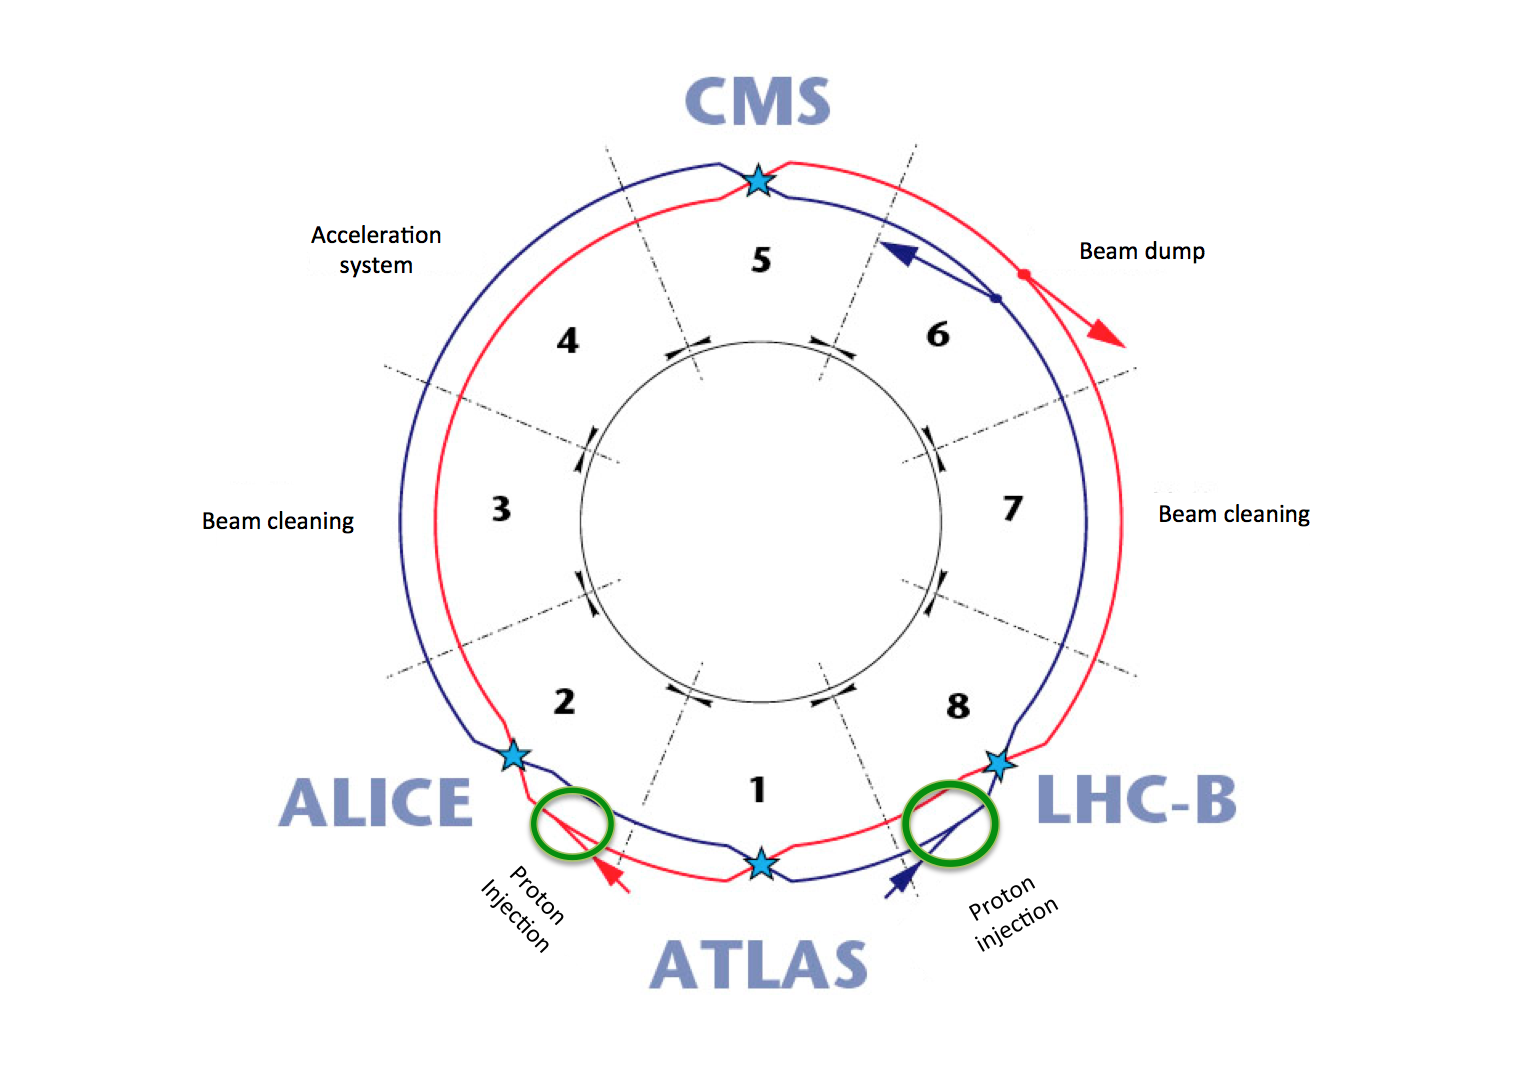
\includegraphics[width=0.75\textwidth]{plots/LHC/LHC_scetch.png}
\caption{Schematic view of the LHC with its eight arcs. The four interaction points, where the experiments are located, are marked with blue stars. Other important parts of the LHC infrastructure are also indicated~\cite{LHCScetch}.}
\label{fig:LHC}
\end{figure}

The protons circulating in the LHC are injected at an energy of $\unit{450}{\giga\electronvolt}$ after running trough a chain of pre-accelerators, the Linac2, the Proton Synchroton Booster (PSB), the Proton Synchrotron (PS), and the Super Proton Synchrotron (SPS). The proton beams are separated into bunches of about $10^{11}$ particles. The smallest temporal spacing between two bunches achieved during the data taking in 2012 was $\unit{50}{\nano\second}$, twice the design value. In these conditions, after three years of running in the years 2010 to 2012, the so called Run I of the LHC, a centre-of-mass energy of $\sqrt{s} = \unit{8}{\tera\electronvolt}$ has been reached. The instantaneous luminosities delivered to the experiments reached a maximum of $\unit{7.7\cdot 10^{33}}{\reciprocal\second\meter\rpsquared}$ in late 2012, as can be seen on the left side of Figure~\ref{fig:lumiOverview}. The integrated luminosity delivered to the CMS experiment in 2012 was $\unit{23.3}{\femto\reciprocal\barn}$, exceeding that of 2011 by almost a factor of four~\cite{LumiTwiki}, as shown on the right side of Figure~\ref{fig:lumiOverview}. 

\begin{figure}[htbp]
\centering
\begin{minipage}[t]{0.49\textwidth}
  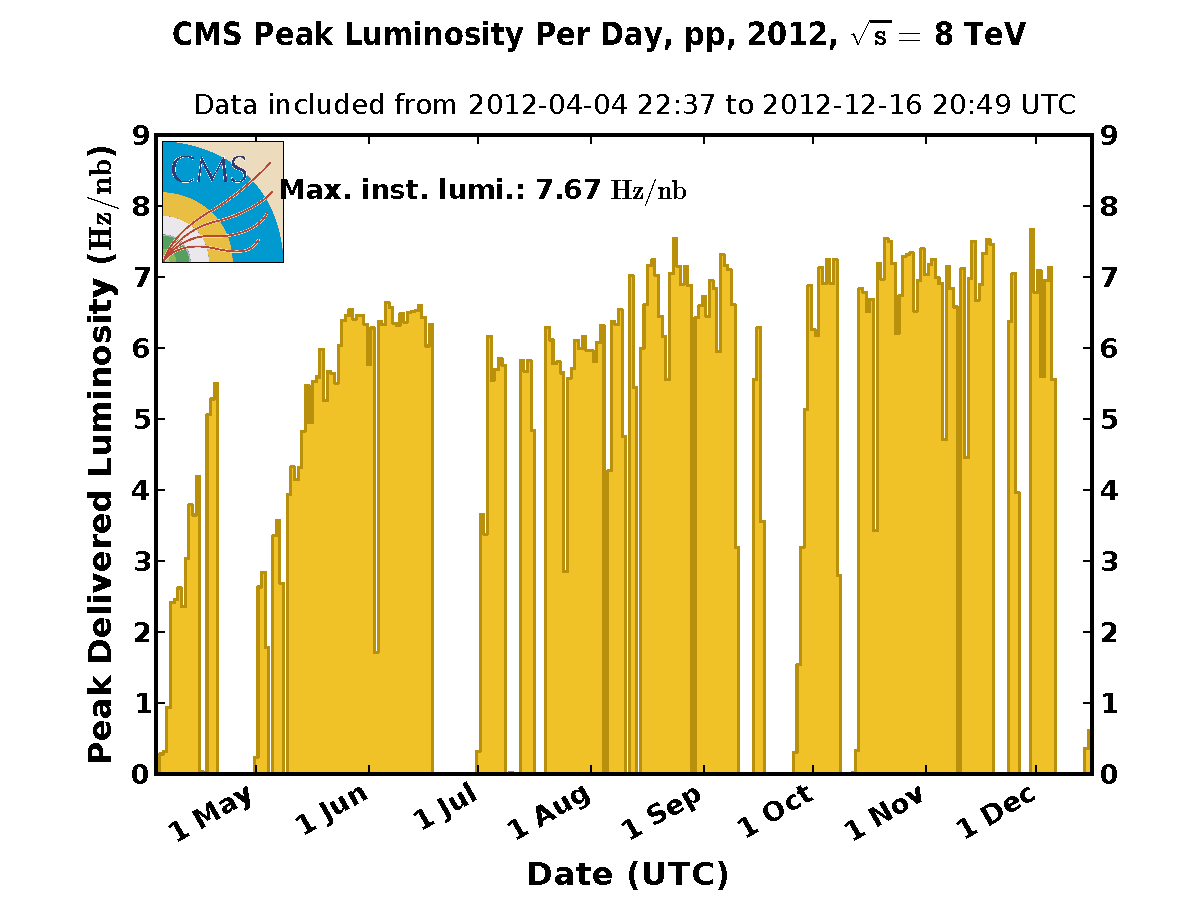
\includegraphics[width=\textwidth]{plots/LHC/peak_lumi_per_day_pp_2012.pdf}
\end{minipage}
\begin{minipage}[t]{0.49\textwidth}
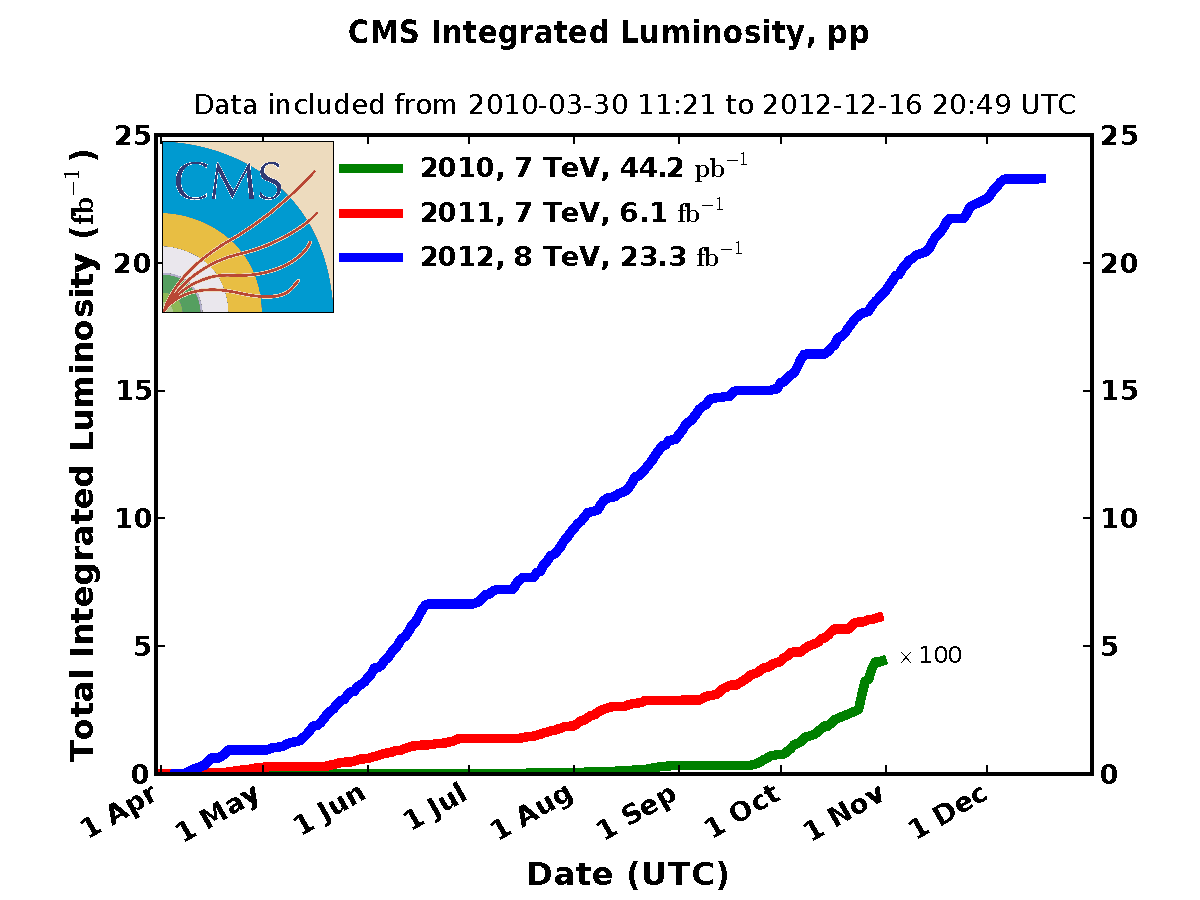
\includegraphics[width=\textwidth]{plots/LHC/int_lumi_cumulative_pp_2.pdf}
\end{minipage}
\caption{Development of instantaneous (left) and integrated (right) luminosity delivered to the CMS experiment. The right plots shows the results for all three years of data taking, while the left one only shows the 2012 data taking~\cite{LumiTwiki}.}
\label{fig:lumiOverview}
\end{figure}